\section{Změna světlosti a kontrastu}
Pro případné odstranění knihovny Cg toolkit z DicomPresenteru, je potřeba nastudovat, zda je možné její funkce nějak realizovat v OpenGL. V případě DicomPresenteru potřebujeme provádět změnu kontrastu a jasu snímku, dále by bylo vhodné v budoucnu implementovat změnu gamma korekce.

Knihovna OpenGL nedisponuje žádnou funkcí pro změnu kontrastu, ale elementárními funkcemi úpravy obrazu vycházejícími ze sčítání a násobení. Abychom zjistili, zda jde změna kontrastu pomocí těchto operací implementovat a dále, zda je taková implementace vyhovující pro běh programu, je potřeba nejdříve nastudovat teorii, co to vlastně změna kontrastu je. Teorii stručně shrnuje první část této sekce, v druhé části je pak rozebrány vlastnosti takové implementace.

\subsection{Světlost a kontrast}
Pro naprogramování funkcí pro změnu světlosti a kontrastu je potřeba nejprve pochopit o jaké matematické operace se jedná. V našem případě se můžeme omezit jen na černobílé snímky, protože výstupem MRI jsou pouze černobílé snímmky. Obrázek tedy můžeme chápat jako matici čísel mezi $0$ a $1$, kde sloupce, respektive řádky odpovídají souřadnicím bodu v obrázku:

\[
 Im_{res_{x},res_{y}} =
 \begin{pmatrix}
  Im(1,1) & Im(1,2) & \cdots & Im(1,res_{x}) \\
  Im(2,1) & Im(2,2) & \cdots & Im(2,res_{x}) \\
  \vdots  & \vdots  & \ddots & \vdots  \\
  Im(res_{y},1) & Im(res_{y},2) & \cdots & Im(res_{y},res_{x})
 \end{pmatrix}
\]

kde \[ Im(x,y) \in [0,1] \]

Pro $ Im(x,y) = 0 $ vidíme pixel naprosto černý, pro $ Im(x,y) = 1 $ vidíme pixel bílý.

Světlost je pak slovně definována jako množství světla jež vyzařuje zdroj. Matematicky přesnější definice pak je:

\emph{Světlost je definována jako střední hodnota světlosti všech bodů.}

Matematicky zapsáno:
\[
  Brightness(Im) = \frac{1}{res_{x}*res_{y}}\sum_{\substack{0 \leq x \leq res_{x} \\ 0 \leq y \leq res_{y}}} Im(x,y)
\]
Změnou světlosti snímku je pak zvětšení, či zmenšení uvedené střední hodnoty. Zpravidla se světlost mění přičtením konstanty ke světlosti všech bodů. Tj. pro bod o souřadnicích $x,y$.
\[
Im(x,y) \longmapsto Im(x,y) + c_{brightness}
\]

Situace s kontrastem snímku je mírně komplikovanější. Kontrast je pro černobílý snímek slovně definován jako rozdíl ve světlosti tmavých a světlých bodů. Tuto vlastnost vystihují nejméně dvě různé definice kontrastu:

Michelsonův kontrast:

\[
Contrast(Im) = \frac{Im_{max}-Im_{min}}{Im_{max}+Im_{min}}
\]

kde:
\[
Im_{max} = \max_{\substack{ 0 \leq x \leq res_{x} \\ 0 \leq y \leq res_{y} }}{Im_{x,y}} 
\]
\[
Im_{min} = \min_{\substack{ 0 \leq x \leq res_{x} \\ 0 \leq y \leq res_{y} }}{Im_{x,y}}
\]

jedná se o jednodušší a názornější definici kontrastu, bohužel však v některých případech neodpovídá pozorovatelným vlastnostem. Takto počítaný kontrast totiž není robustní vůči výchylkám jednotlivých bodů. Představme si snímek $1000*1000$ bodů, kde světlost téměř všech bodů se bude pohybovat mezi hodnotami $0.4$ a $0.6$, světlost jednoho bodu bude $0$ a světlost dalšího bodu bude $1$. V tomto případě je kontrast snímku $1$. Po přeškálování světlosti uvedených dvou bodů na hodnotu $0,5$ se rázem změní kontrast snímku na hodnotu $0,2$. Přitom jsme během změny kontrastu na snímku nemohli pozorovat prakticky nic.

Vhodnější definice kontrastu by tedy byla následující:

Root Mean Square Contrast:
\[
Contrast(Im) = \sqrt{\frac{1}{res_{x}*res_{y}}\sum_{\substack{ 0 \leq x \leq res_{x} \\ 0 \leq y \leq res_{y} }}(Im_{x,y}-Brightness(Im))^2}
\]

Vzorec pro výpočet kontrastu nápadně připomíná výpočet rozptylu náhodné veličiny. 

Při porovnání obou vzorců vidíme, že první vzorec je velice jednoduchý na výpočet, ale výsledek přesně nevystihuje vizuální dojem z obrázku. Druhý výpočet je výrazně náročnější na výpočet, ale je také nesrovnatelně přesnější. Jako vhodná alternativa se tak nabízí používat druhý vzorec, ale do sumy dosadit pouze náhodný výběr bodů z obrázku.

Změna kontrastu snímku se ve většině počítačových programů provádí podle následujícího pravidla pro světlost bodu:
\[
  Im(x,y) \longmapsto   (Im(x,y) - 0.5)*c_{contrast} + 0.5
\]

Původní hodnotu svělosti pixelu zmenšíme o $0.5$. Díky tomuto kroku pak při násobení získané hodnoty koeficientem $c_{contrast}$ docílíme toho, že pixely s původní světlostí pod $0.5$ získají ještě nižší hodnotu světlosti, naopak pixely se světlostí nad $0.5$ získají vyšší světlost. Dále přičteme hodnotu $0.5$ a tím se vrátí hodnoty světlosti na původní úroveň.

Nejlépe je pak vidět uvedená transfmormace, když si její transformační křivku. Na transformaci $ Cont(*,c_{contrast}) $ se můžeme dívat jako na funkci jedné proměnné na intervalu $[0,1]$. Pro vstupní hodnotu $ Im(x,y) $ získáme výstupní hodnotu $ (Im(x,y) - 0.5)*c_{contrast} + 0.5 $.

Pro $ c_{contrast}=1 $, tedy pro transformaci, jež zachová obrázek v původním stavu, bude graf funkce $ Cont(*,c_{contrast}) $ vypadat následovně:

%\begin{figure}[here]
\begin{center}
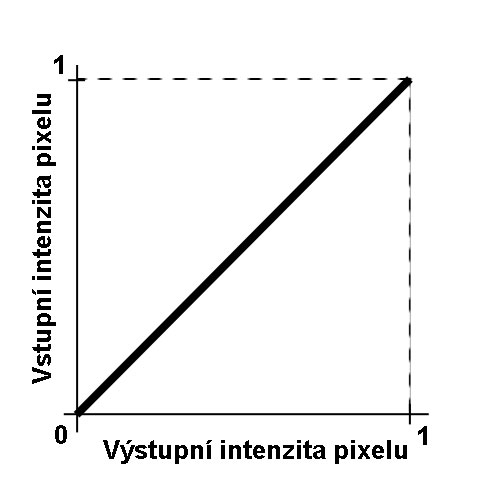
\includegraphics[width=0.7\textwidth,height=0.7\textwidth]{Text/IMG/Kontrast_Identita.jpg}
\end{center}
%\caption{Křivka znázorňující barevnou transformaci, při které se snímek nezmění.}
%\label{kontrastKrivka}
%\end{figure}

Pixel o vstupní intenzitě $0.25$ bude mít výstupní intenzitu $0.25$.

Ukažme si nyní, jak vypadá stejná křivka pro transformaci, která kontrast obrázku zvyšuje, např. pro $ c_{contrast}=1.25 $.
Vezmeme-li v úvahu uvedený vzorec a vezmeme-li dále v úvahu podmínku $ Im(x,y) \in [0,1] $.

Pak můžeme křivku transformace pro $ c_{contrast}=1.25 $ načrtnout takto:


%\begin{figure}
\begin{center}
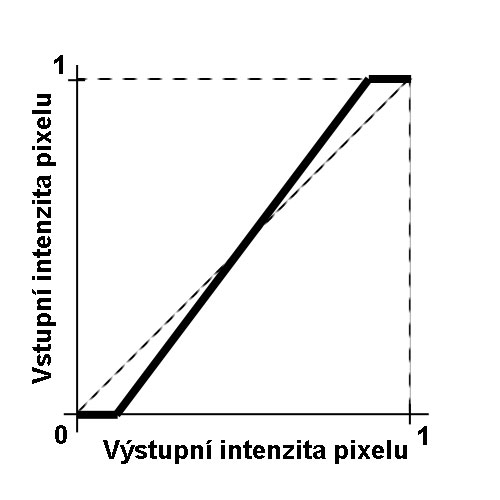
\includegraphics[width=0.7\textwidth,height=0.7\textwidth]{Text/IMG/Kontrast_Transformace_1.jpg}
\end{center}
%\caption{Transformační křivka změny kontrastu.}
%\label{kontrastKrivka}
%\end{figure}

Křivka na obrázku má strmější spád. To znamená, že světlejší pixely (s původní světlostí $> 0.5$) se staly ještě světlejší a naopak tmavší pixely (s původní světlostí $< 0.5$) ještě více ztmavly. Z uvedeného nákresu je pak vidět co vyplývá z předpisu transformace a podmínek $ Im(x,y) \in [0,1]$. Při zvýšení kontrastu koeficientem k se intenzita všech bodů, jejichž intenzita je z intervalu $ [0,\frac{1}{2k}] $, změní na $0$ a dále intenzita všech bodů, jejíchž původní intenzita byla v intervalu $[1-\frac{1}{2k},1]$, se změní na hodnotu $1$. Jinými slovy, jak se v odborné terminologii užívá, dojde ke ztrátě grafické informace a to v uvedených množinách bodů. Volnější parafrázi bychom řekli, že odstíny největlejší bodů se slijí do jediného odstínu a odstíny nejtmavších bodů se slijí do jediného odstínu (viz tabulka \ref{highcontrast}).

\begin{table}%[ht]
	\caption{Příklad příliš výrazné změny kontrastu, kdy dochází ke ztrátě grafické informace.}
\label{highcontrast}
		\begin{tabular}{p{7cm}p{7cm}}
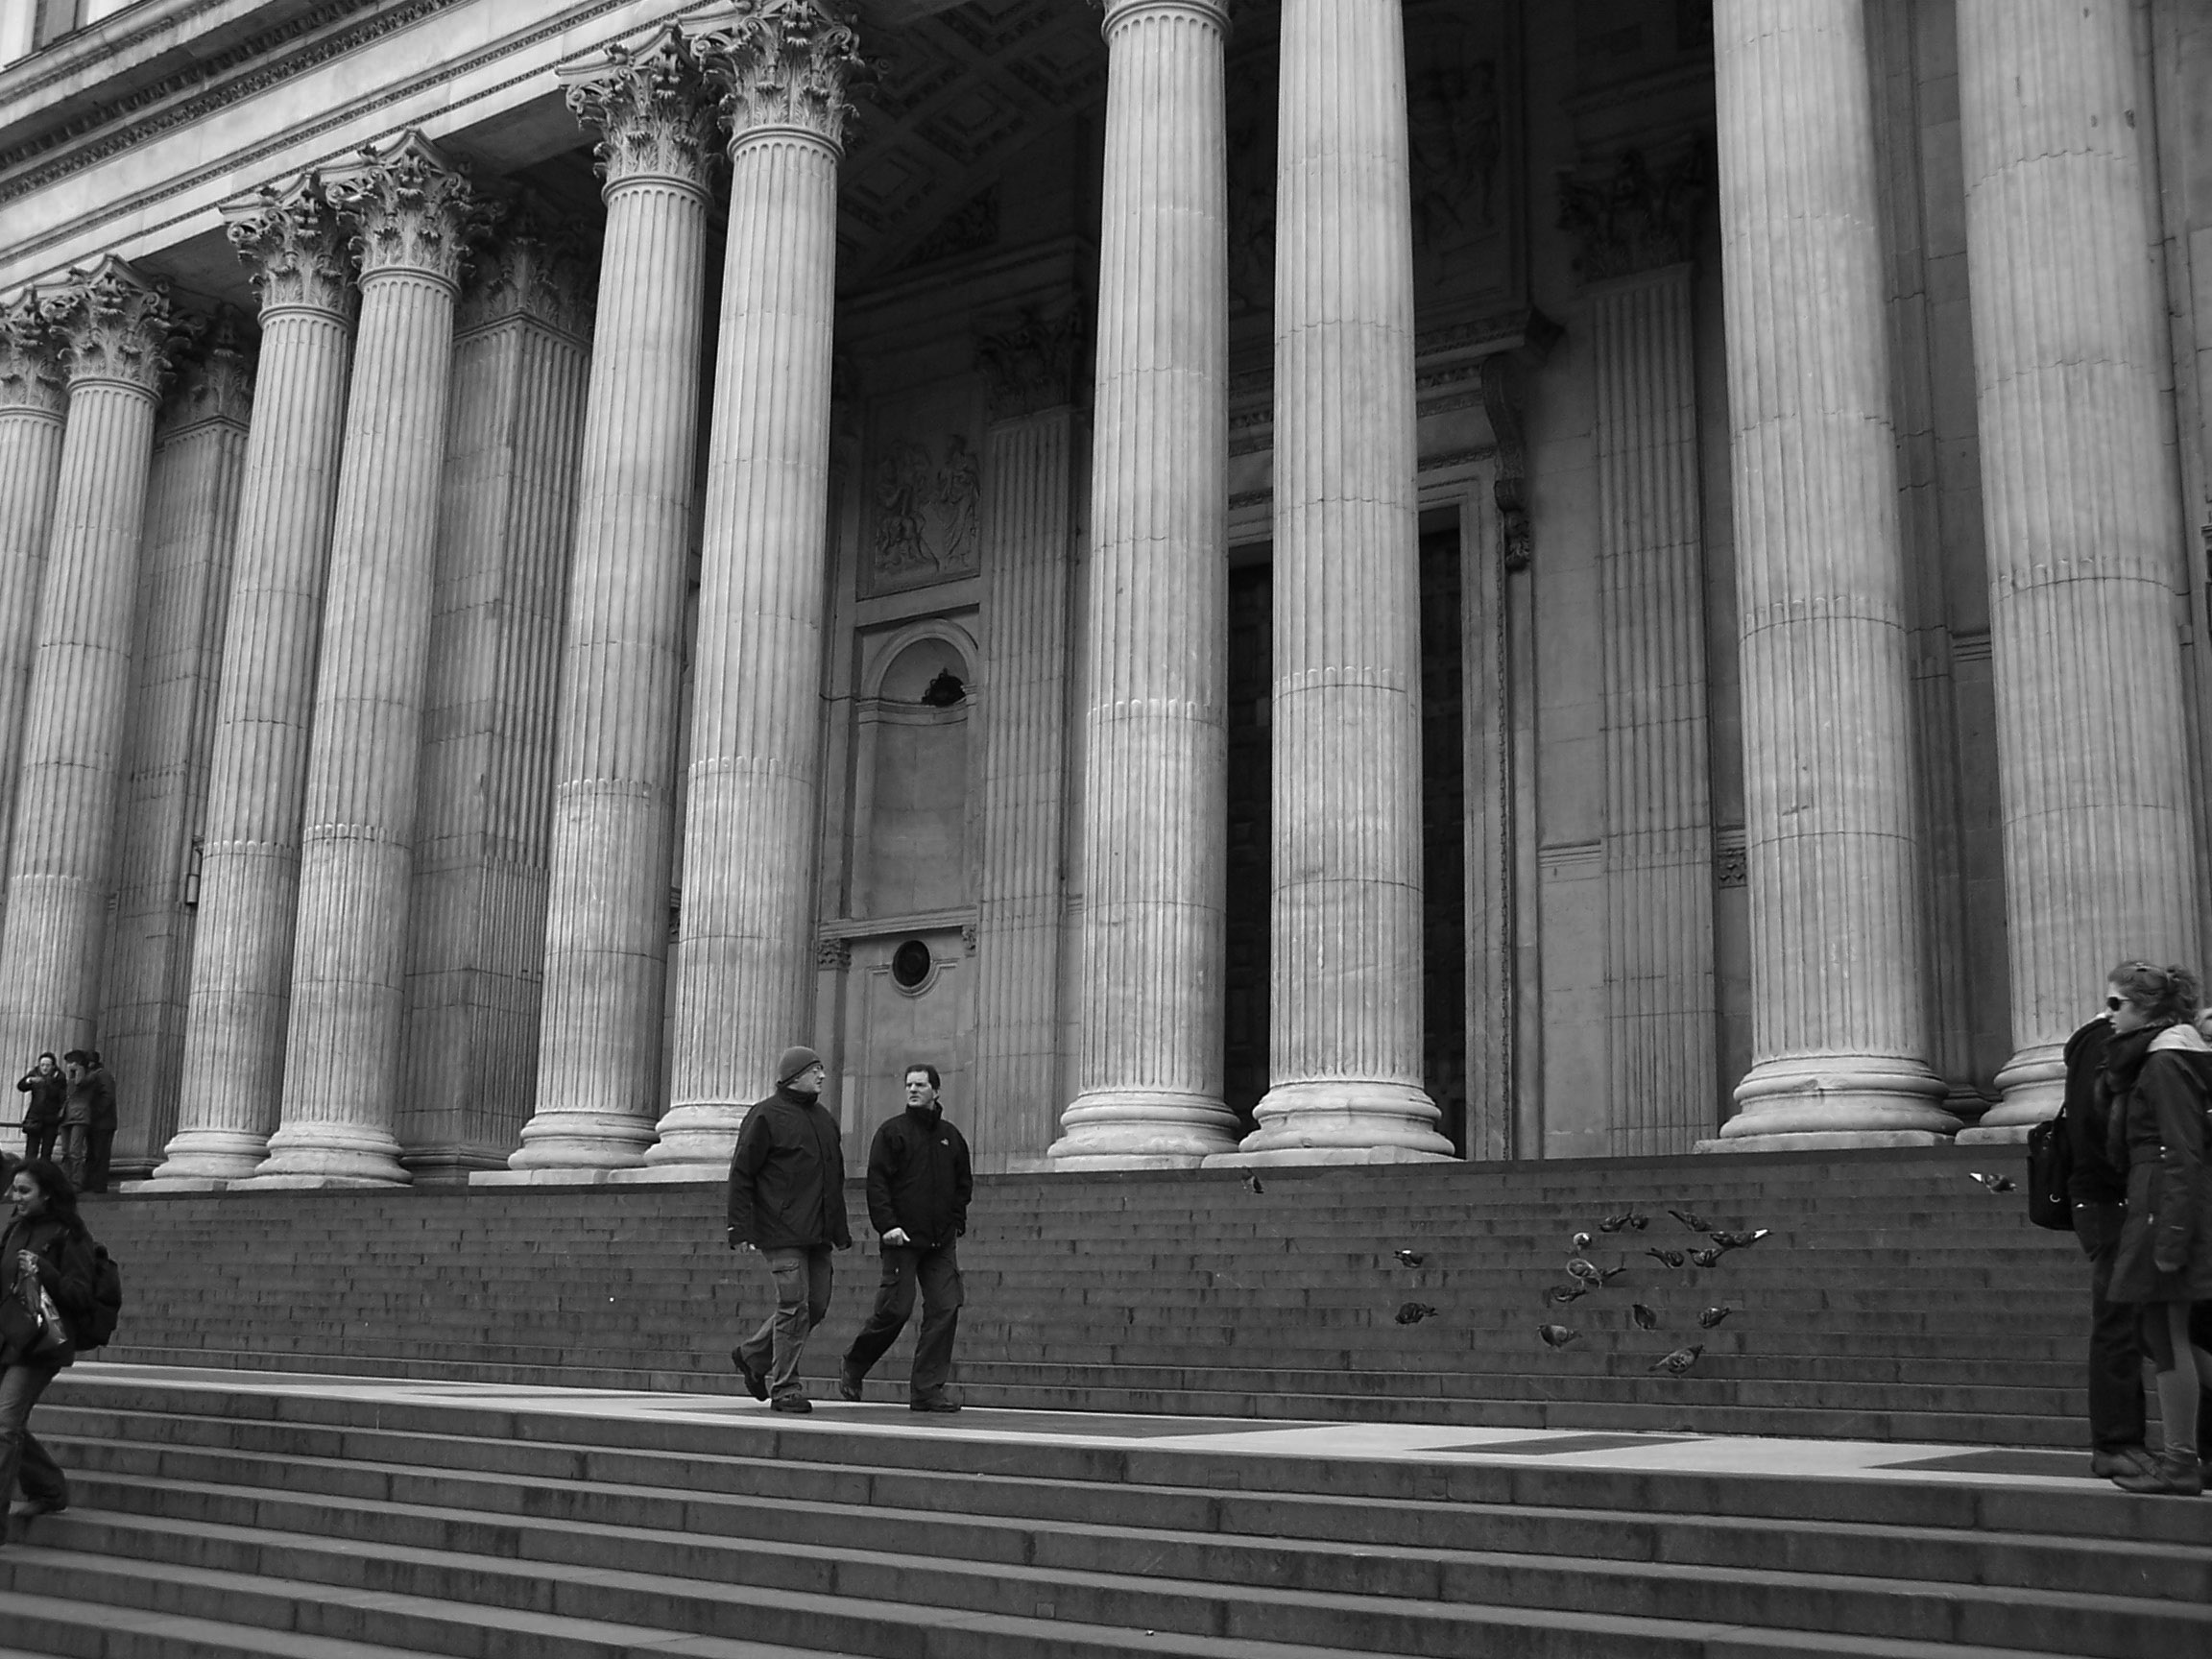
\includegraphics[width=0.5\textwidth,height=0.35\textwidth]{Text/IMG/London.jpg} & 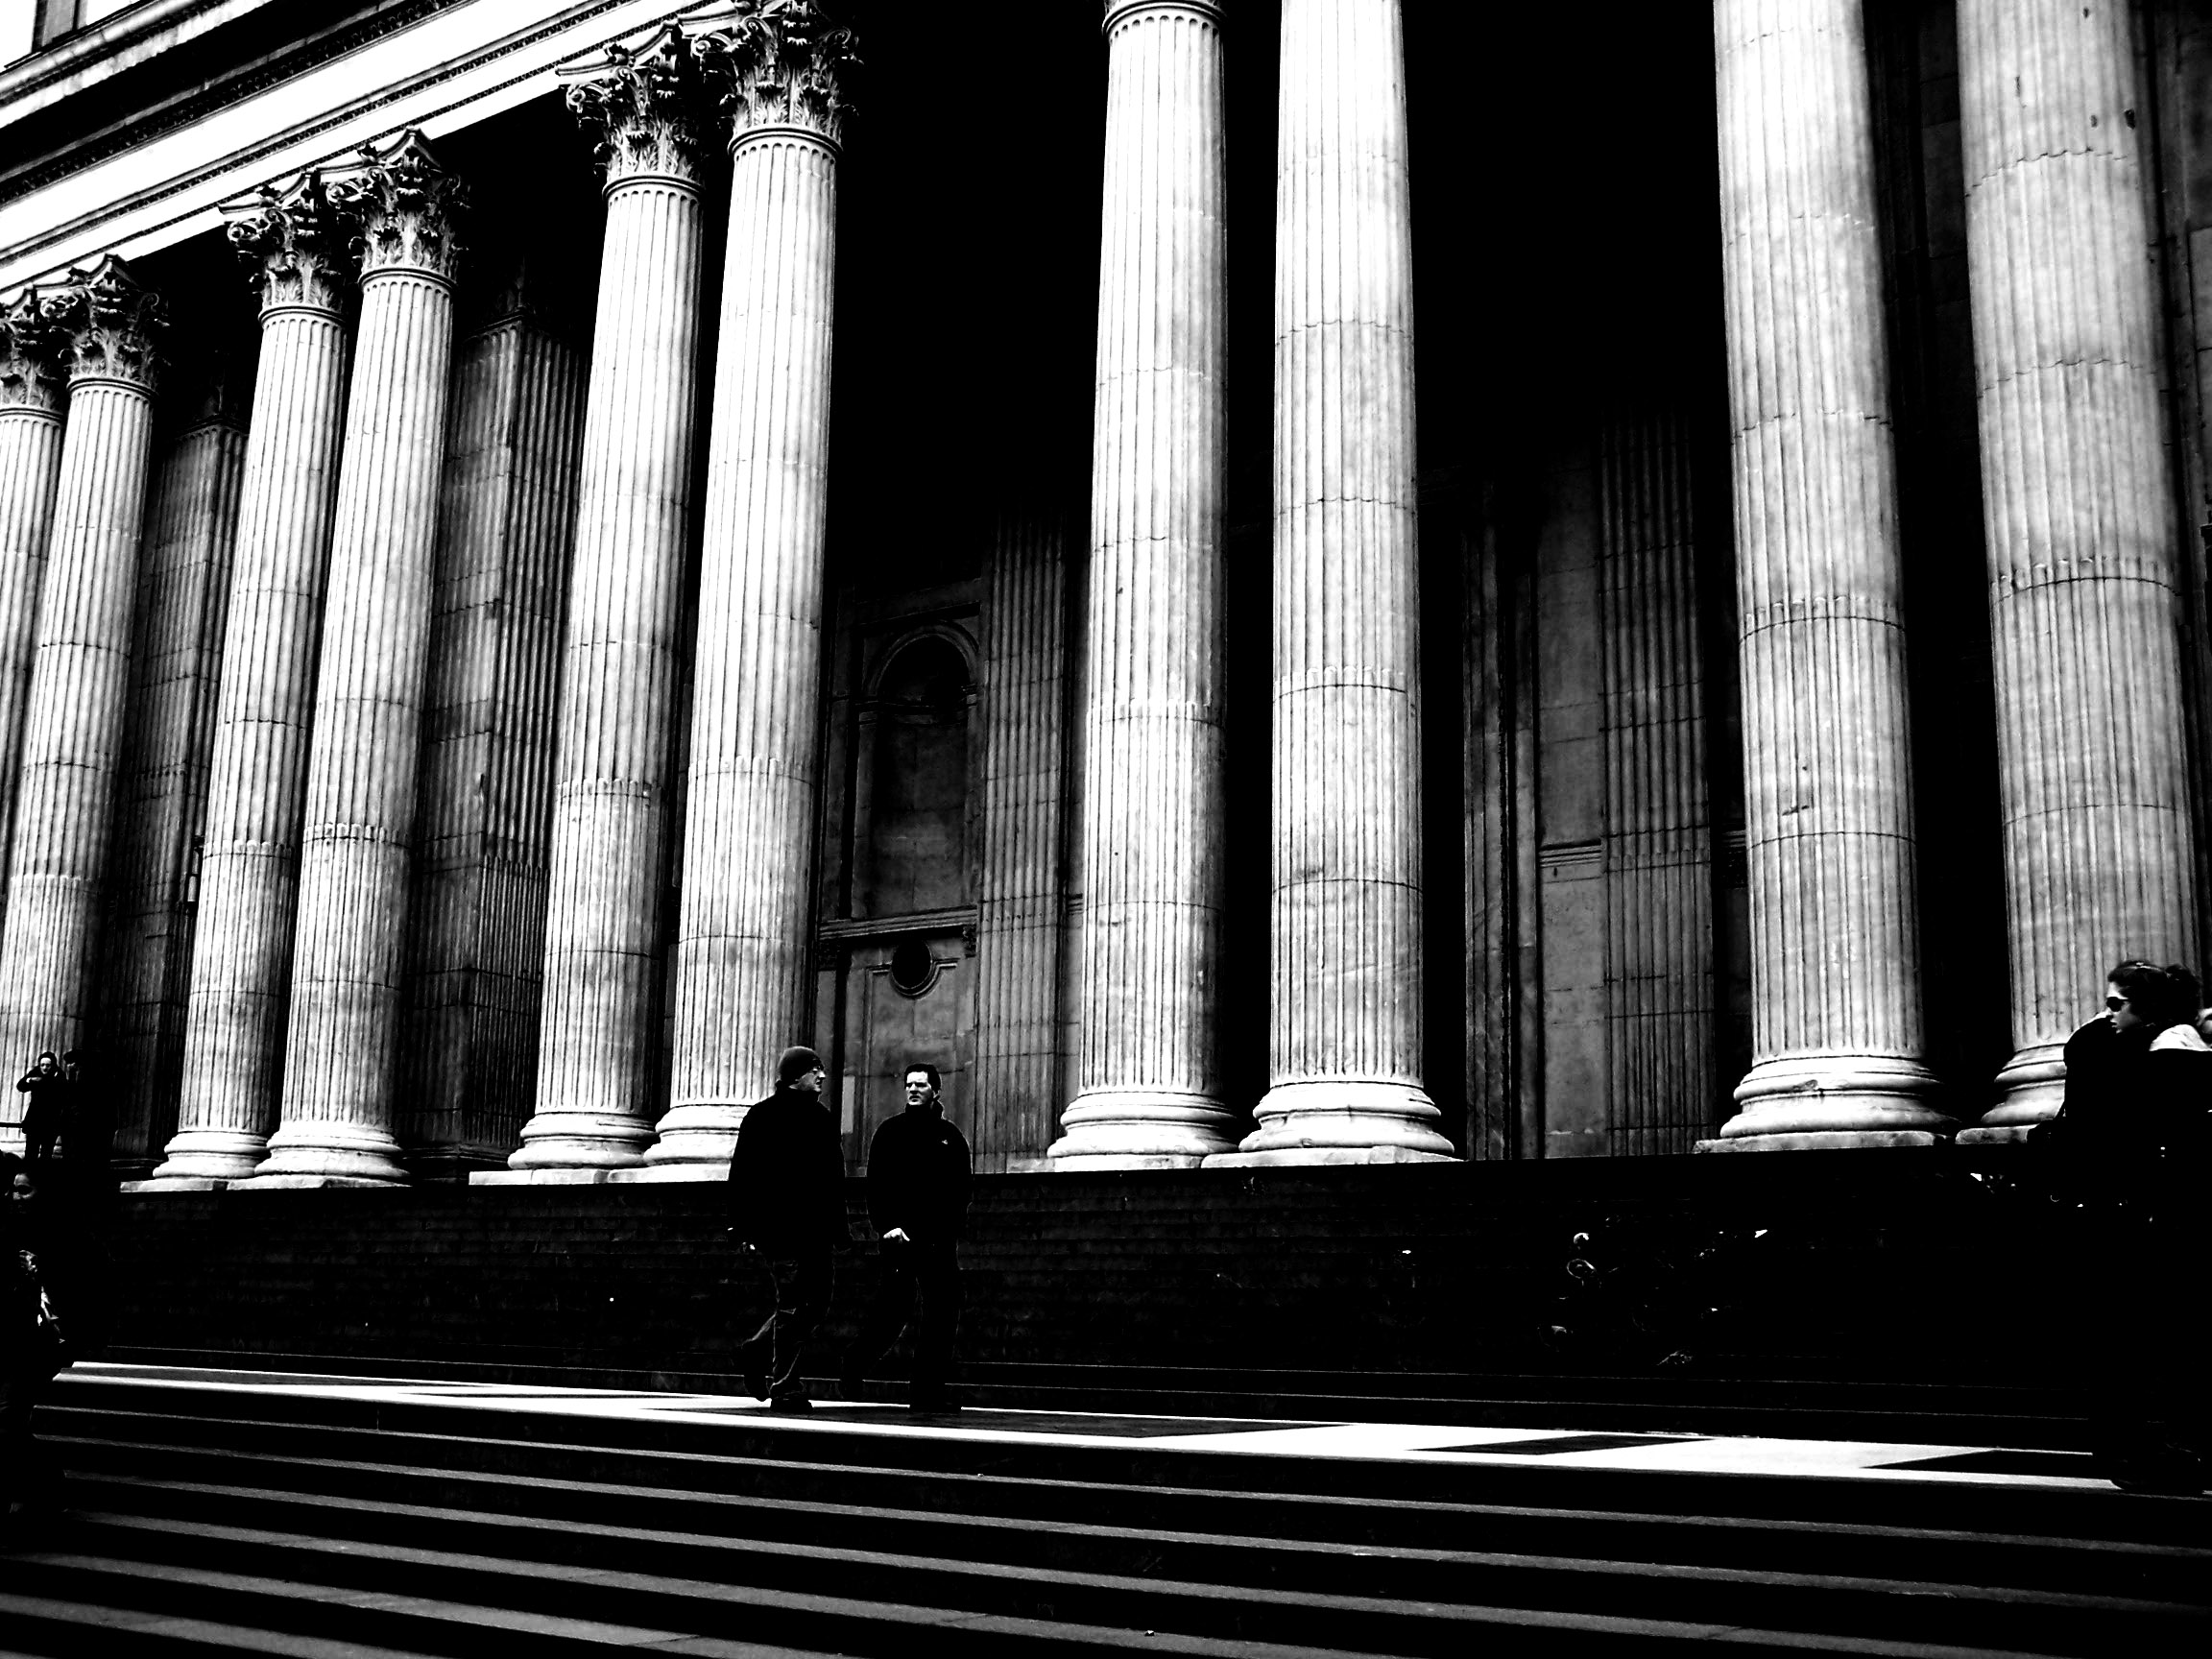
\includegraphics[width=0.5\textwidth,height=0.35\textwidth]{Text/IMG/London_High_Contrast.jpg} \\
\center{Původní obrázek.} & \center{Obrázek po změně kontrastu.}\\
		\end{tabular}
\end{table}

Nejmodernější počítačové programy pak používají nelineární transformace pro změnu kontrastu. Při jejich použití nedochází ke ztrátě grafické informace. Křivka takové transformace pak vypadá přibližně takto: 

\begin{center}
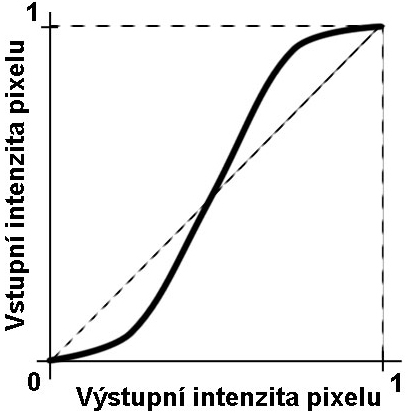
\includegraphics[width=0.7\textwidth,height=0.7\textwidth]{Text/IMG/Kontrast_Transformace_2.jpg}
\end{center}





\newpage
\subsection{Kontrast a světlost v OpenGL}
Pro grafické operace disponuje knihovna OpenGL s funkcemi Bias a Scale. Po bližším nastudování obou funkcí lze zjistit, že přirozeně vychází z matematických funkcí sčítámí a násobení.

\begin{itemize}
\item Voláním funkce Scale s parametry K,B provedeme přičtení konstanty K k hodnotě barevné složky B a to pro všechny pixely obrázku.
\item Voláním funkce Bias s parametry K,B provedeme vynásobení stávající barevné složky B konstantou K a to pro všechny pixely obrázku.
\end{itemize}

Podíváme-li se na křivku barevné transformace při volání funkce Bias s parametrem 1,5 bude křivka vypadat takto:

\begin{center}
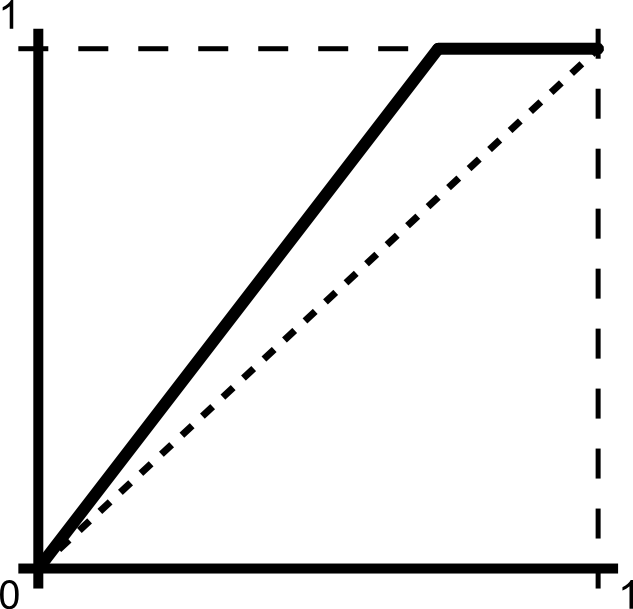
\includegraphics[width=0.5\textwidth]{Text/IMG/Bias.png}
\end{center}

Výsledek lze interpretovat tak, že parametr Bias mění směrnici transformační křivky, nemění však její posunutí.

Transformační křivka pro změnu kontrastu ale vždy prochází bodem [ 0,5 ; 0,5 ]. Křivku z předchozího obrázku tak musíme o konstantu posunout.

Přičítání konstanty k hodnotě barevné složky pro všechny pixely obrázku tak jak to provádí funkce Scale právě odpovídá posunutí křivky transformace.

Podíváme-li se na transformační křivku po volání funkce Scale s parametrem 0,25, bude vypadat takto:

\begin{center}
\includegraphics[width=0.5\textwidth]{Text/IMG/Scale.png}
\end{center}

Jak lze vydedukovat z vlastností u obou příkladů, zkombinujeme-li obě transformace, tj. změníme-li směrnici transformační křivky grafu a posuneme-li ji o správnou hodnotu, lze dosáhnout transformace, která odpovídá změně kontrastu.

Volme parametry:

Bias = 1.2
Scale = -0.1

Pak graf bude vypadat:

\begin{center}
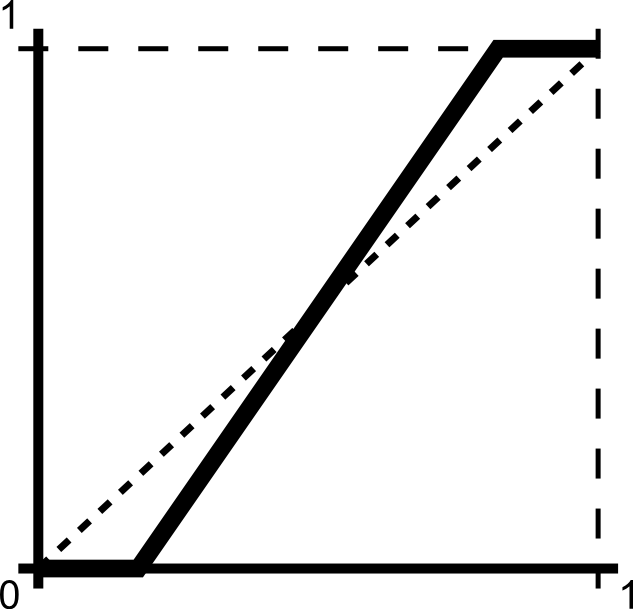
\includegraphics[width=0.5\textwidth]{Text/IMG/BiasScale.png}
\end{center}

Tato transformační křivka přesně odpovídá jednodušší (často implementované) variantě změny kontrastu.



\subsection{Kontrast v knihovně Cg}
Knihovna Cg toolkit nám nabízí programování vlastních výpočtů s barvou pixelů. Paleta možných transformací je pak velice široká a implementace je jednoduchá - program napíšeme v jazyku Cg, který je velice podobný jazyku C.

Implementace změny kontrastu pak bude vypadat:
\begin{lstlisting}[label=DicomImageClass,caption={...}]
C3E3f_Output main(float2 texCoord : TEXCOORD0, uniform sampler2D decal : TEX0, uniform float brightness){
  C3E3f_Output OUT;
  OUT.color = tex2D(decal,texCoord)*bias - scale;
  return OUT;
}
\end{lstlisting}

Ve srovnání s OpenGL je tato implementace výrazně přehlednější. Podíváme-li se na řádek 3, vidíme hned zápis transformační funkce ve tvaru: f(x) = k*x - z. Jak již lze předpokládat: s jazykem Cg můžeme jednoduše popisovat mnohem složitější transformace využívající elementárních matematických funkcí: log, exp, sin.




\subsection{Závěr}
Z programu DicomPresenter je možné odstranit knihovnu Cg. Omezíme-li se v programu na použití pouze elementárních obrazových transformací: kontrast a jas, můžeme tyto implementovat i v OpenGL. Důvodem, proč je v programu použita knihovna Cg toolkit, bylo v práci \cite{neskudla} uvedeno, že bez ní dojde při vícenásobné transformaci oříznutí barev obrázku: když kontrast hodně zvýšíme a opět snížíme, vytrarí se z obrázku část původní informace. Toto však lze obejít, uložíme-li si snímek do paměti dvakrát: původní s nezměněným kontrastem a výsledný po změně, který zobrazíme uživateli. Bude-li si přát uživatel další změnu kontrastu, nebudeme jí počítat ze snímku, který vidí, ale z původního, jež je uložen v paměti. Nevýhoda tohoto řešení je ta, že pro dvojrozměrné snímky budeme zatěžovat operační paměť dvojnásobkem dat. Vzhledem k tomu, že snímky jsou uloženy v paměti grafické karty je toto omězení poměrně vážné (pro starší grafické karty).


